\subsection{Product Perspective}

\subsubsection{Class Diagram}
%%%%%%%%%%%%%%%%%%%%%%%%%%%%%%%%%%%
%%%%%%%%% CLASS DIAGRAM  %%%%%%%%%%
%%%%%%%%%%%%%%%%%%%%%%%%%%%%%%%%%%%

\begin{figure}[bht!]
\centering
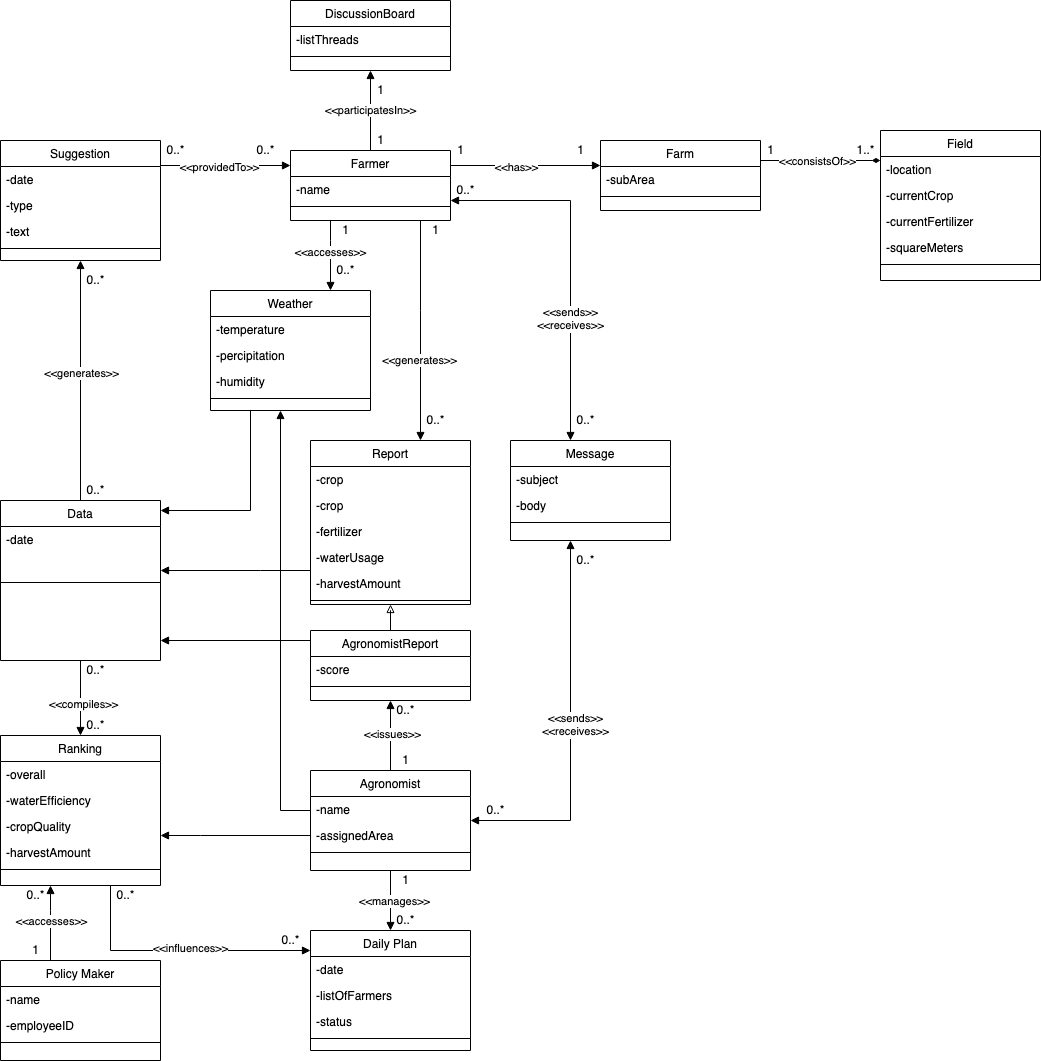
\includegraphics[scale=0.35]{../images_diagrams/class_diagram.drawio.png}
\caption{\label{fig:classdiagram}Class diagram.}
\end{figure}

\begin{flushleft}
The UML class diagram shown in \textbf{Figure \ref{fig:classdiagram}} shows a simplified view of the classes needed to support the functions expected from the system. This is not a comprehensive view of all the classes needed but rather a focused view to capture the general decomposition of the different classes and the different relations between them. Considering the goals described in Section \ref{goalsection}, the main features that DREAM delivers include a discussion board for farmers to seek support, a messaging interface for farmers and agronomists to communicate, reports for farmers and agronomists to log data, a daily plan interface for agronomists to manage their visits, a visualization of performance for agronomists and policy makers to access, and a suggestion generator for farmers. The classes and the relations included in \textbf{Figure \ref{fig:classdiagram}} are derived from these main features. The classes are described in detail:

%%%%%%%%%%%%%%%%%%%%%%%%%%%%%%%%%%%
%%%%%% DESCRIPTION OF CLASSES %%%%%
%%%%%%%%%%%%%%%%%%%%%%%%%%%%%%%%%%%
\begin{itemize}

\item \textbf{Farmer}\\
The Farmer class corresponds to a farmer user. The class should have access to all the functions necessary to support the use cases related to a farmer user. 

\item \textbf{Farm}\\
The Farm class corresponds to a farm. As demonstrated by the class diagram, each instance of the Farm class is managed by one Farmer. The Telangana region is split into multiple subareas therefore the Farm class is associated with a subarea instead of GPS location.

\item \textbf{Field}\\
The Field class is distinct from the Farm class to enable a farmer to manage physically disjoint properties. Each farm is made up of one or more fields. Each field has its own GPS location as well as other agriculture-specific attributes.

\item \textbf{Report}\\
The FarmerReport class is related to the Farmer class because farmers can submit reports with data describing the status of their fields in order to maintain a historical record of their progress. 

\item \textbf{DiscussionBoard}\\
The Farmer class also interacts with the DiscussionBoard class to indicate that the farmer user can interact with the discussion board. For simplicity, other classes that support the implementation of the forum, such as a Thread class or a Post class, are abstracted into DiscussionBoard. 

\item \textbf{Agronomist}\\
The Agronomist class corresponds to an agronomist user. The class should have access to all the functions necessary to support the use cases related to an agronomist user. 

\item \textbf{AgronomistReport}\\
The AgronomistReport class extends from the FarmerReport class that is used by the Farmer class. The difference is that the AgronomistReport also includes a numerical score issued by the agronomist user. 

\item \textbf{DailyPlan}\\
The DailyPlan class is related to the Agronomist class because the plans created are specifically for agronomists. This class includes all the functions necessary to support an agronomist user managing their daily plan such as viewing the route, modifying the farmers included in the plan, or entering reports for each farmer visit. Again, the other classes necessary to support the implementation of these functions are abstracted into DailyPlan.

\item \textbf{Weather}\\
The Weather class is related to both the Farmer class and the Agronomist class because both the farmer user and agronomist user need to access weather information. Again, other classes necessary to implement an interface to visualize weather data such as in a map view are abstracted out for simplicity.
\smallskip\\
Since the Agronomist class is associated with an assigned subarea, the class diagram omits an Area class and relates the Agronomist class with the Weather class directly. Similarly, since the Farmer is associated with the GPS location through their Farm and Field classes, the Farmer class can relate to the Weather class directly. 

\item \textbf{Message}\\
The Message class is related to the Farmer class and the Agronomist class because both the farmer users and the agronomist users can send and receive messages to each other. Again, other classes that may be necessary to implement the messaging feature are ommited from this diagram for simplicity.

\item \textbf{Data}\\
The Data class aggregates data from the Weather class, the Report class, and the AgronomistReport class. This class performs some data processing and sends it to the Suggestion and Ranking classes, hence the relations in the diagram. 

\item \textbf{Suggestion}\\
The Suggestion class is related to the Farmer class because personalized suggestions are auto-generated and issued to farmers based on the data aggregated in the Data class.

\item \textbf{Ranking}\\
The Ranking class is related to the PolicyMaker class because policy makers must access ranking views of the farmers. The Ranking class is also related to the Agronomist class because agronomists must also access ranking views of the farmers, but their view is limited to the farmers in their subarea. These configurable ranking views are based on the data aggregated in the Data class. This ranking influences the priority farmers are given when scheduling the daily plans for agronomists, therefore the Ranking class is related to the DailyPlan class.

\item \textbf{PolicyMaker}\\
The PolicyMaker class corresponds to a policy maker user. The class should have access to all the functions necessary to support the use cases related to a policy maker user. 

\end{itemize}
\end{flushleft}

%%%%%%%%%%%%%%%%%%%%%%%%%%%%%%%%%%%
%%%%%%%% PRODUCT FUNCTIONS %%%%%%%%
%%%%%%%%%%%%%%%%%%%%%%%%%%%%%%%%%%%


\subsection{Product Functions}
\begin{flushleft}

Below is a detailed description of all the main functions of the product. The product functions are generalizations of the specific goals of the product. The functions are further specified in the requirements section and select functions are demonstrated in the scenarios section. 

\subsubsection{Data Visualization}
DREAM helps the farmers to visualize and analyze data about their production: providing simple graphs and statistics to the users, the application allows them to better understand their needs. In the section named "My Farm" each user can find personalized suggestions: thanks to the data provided by the farmers, DREAMS can recommend the type of crop to plant or the best fertilizer to use. DREAMS also provides the users a precise weather forecast that is updated daily.

\subsubsection{Support for Farmers and Discussion Forums}
With DREAM, each farmer can easily ask for help or suggestions directly from professional agronomists: inside the "Ask experts" section, the user can send messages to agronomists and obtain vital information to improve their production. Another opportunity is the "Farmers Forum" where each farmer can ask for help from other farmers or read answers to already posted questions.

\subsubsection{Performance Visualization and Evaluations}
The DREAM system offers agronomists and policy makers a visualization of the performance of the farmers by means of a ranked list view. Agronomists only visualize the performance of the farmers inside their responsible area whereas policy makers can visualize the performance of all the farmers involved in the DREAM initiative. By default, this visualization of the ranking organizes farmers by their overall score which combines data such as crop quality, production yields, water usage, and evaluations by the agronomists. Users can configure their ranking view to filter by one of these metrics, by location, or by other attributes of the farmers. \\
\smallskip
In addition to a visualization of performance, policy makers can also access evaluations of the farmers issued by agronomists that enable the policy makers to determine the efficacy of the support provided to the farmer. 

\subsubsection{Daily Plan}
The DREAM system provides the agronomists a tool for managing their daily plans with functions such as plan creation, modification, and confirmation. During the creation of the daily plan, the system recommends farmers to visit based on the performance of the farmers and the and frequency of visits. The system also displays a map containing all the fields of the farmers. As the agronomist modifies their list of farmers to visit as part of the daily plan, the DREAM system updates the travel path connecting the fields. During the confirmation of the daily plan, the system allows the agronomist insert all the data about the visits they performed during the day.
\end{flushleft}


%%%%%%%%%%%%%%%%%%%%%%%%%%%%%%%%%%%
%%%%%%% USER CHARACTERISTICS %%%%%%
%%%%%%%%%%%%%%%%%%%%%%%%%%%%%%%%%%%


\subsection{User Characteristics}
\begin{flushleft}
Users of the system fall into one of the following categories: farmer, agronomist, or policy maker.
\subsubsection{Farmer}
A farmer is the type of user that intends to use the DREAM system to visualize data relevant to them such as: weather forecasts or personalized suggestions. Personalized suggestions generated by the DREAM product may consist of new crops to consider planting, different fertilizers to use, or other cultivation methods to try. Farmers can also use the DREAM system to ask professional agronomists and other nearby farmers for help and suggestions.\\
\subsubsection{Agronomist}
An Agronomist is a type of user that intends to use the DREAM system as a tool to manage some of their job responsibilities. Agronomists want to: receive requests for help from the farmers; answer requests from farmers; inspect rankings of the performance of farmers; provide evaluations regarding farmers performance; and utilize a tool to create, modify and confirm daily plans to manage farms visits.
\subsubsection{Policy Maker}
A Telangana policy maker is a type of user that intends to use the DREAM system to drive policy decisions. Policy makers are mainly interested in accessing rankings and evaluations of all the farmers in the entire area as well as identifying broader trends in the data such as relating the community-provided support to production outcomes. Since policy makers have a more holistic view of the region, they use the DREAM system to configure metrics that are used to classify "well-performing" and "poor-performing" farmers based on rankings, evaluations, and data.\\
\end{flushleft}



%%%%%%%%%%%%%%%%%%%%%%%%%%%%%%%%%%%
%%%%%%%%%%% FLOWCHARTS %%%%%%%%%%%%
%%%%%%%%%%%%%%%%%%%%%%%%%%%%%%%%%%%
\subsection{Flowcharts}


\begin{figure}[hbt!]
\centering
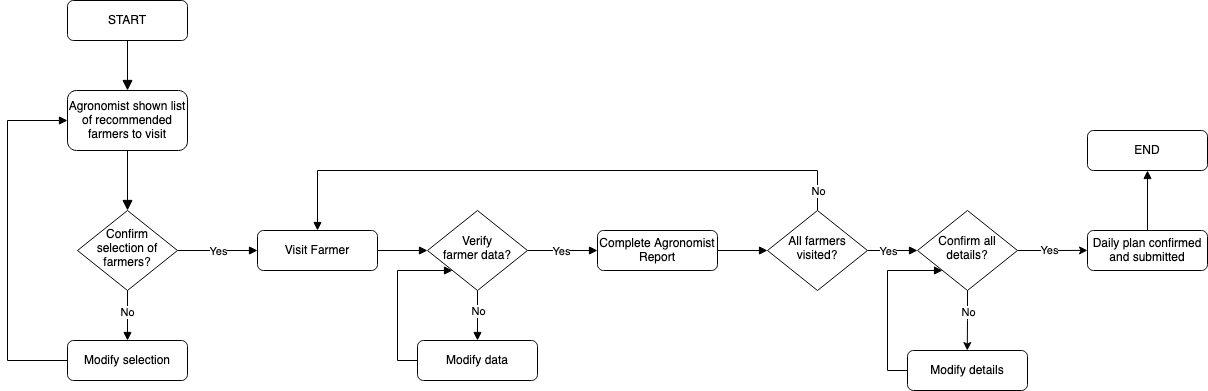
\includegraphics[scale=0.4]{../images_diagrams/agronomistexecutesplan.png}
\caption{\label{fig:flowAgronomistReport}Daily plans flowchart.}
\end{figure}

\begin{flushleft}
The UML flowchart in \textbf{Figure \ref{fig:flowAgronomistReport}} describes the correlation between the agronomist user and the farmer user when the agronomist launches the interface to start a new daily plan. It shows the process of the agronomist entering their reports as they visit the farmers in their plan.In the beginning of the flow, the agronomist can manually modify the farmers they are scheduled to visit that day. Then for each farmer the agronomist visits, the agronomist generates a report to capture a snapshot of the farmer's status. After visiting all the farmers scheduled, the agronomist must confirm all the details such as ensuring that all the reports are complete and all the farmers that were in fact visited are included. After confirming, the daily plan is submitted into the system.
\end{flushleft}

\begin{figure}[hbt!]
\centering
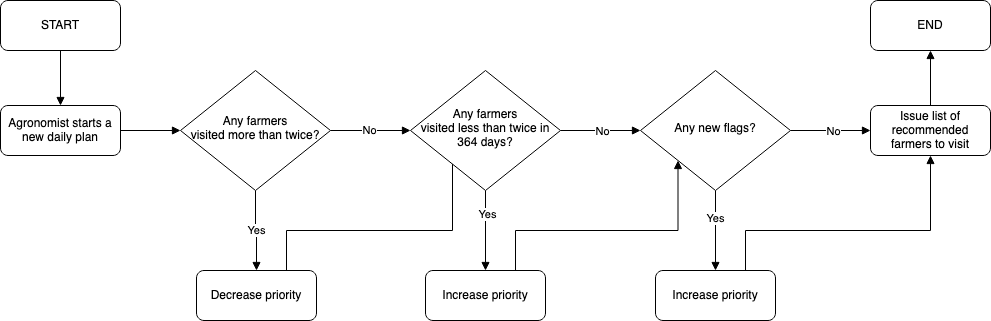
\includegraphics[scale=0.4]{../images_diagrams/adjustvisitpriority.png}
\caption{\label{fig:flowPriority}Farmer priority flowchart.}
%\caption{\label{fig:flowPriority}This flowchart gives a general sense of how DREAM determines the priority for the farmers when providing agronomists a list of recommended farmers to visit for that day.}
\end{figure}


\begin{flushleft}
The UML flowchart in \textbf{Figure \ref{fig:flowPriority}} goes into more detail about how the other elements in the system affect the method in which farmers are chosen when the agronomist launches a new daily plan. The general mandate is that farmers must be visited at least twice a year, therefore the first pass deprioritizes farmers who have been visited more than twice in the last year. Then, there is a check to increase the priority for farmers that have not yet met the twice-a-year minimum. Specifically, this pass looks for farmers where it would be the last day to satisfy the minimum. The last pass increases the priority for farmers who have been flagged, either manually by policy makers or automatically by the triggers set in the system. This flowchart does not detail the specific way in which the farmer visiting queue is generated but instead gives a high-level view of the other elements of the system that contribute to the calculation of the priority. 
\end{flushleft}


\newpage


\begin{figure}[hbt!]
\centering
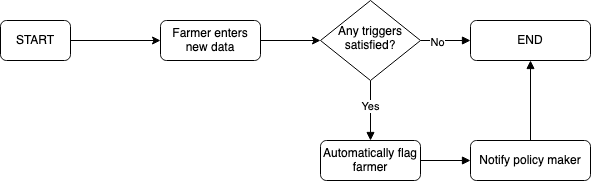
\includegraphics[scale=0.4]{../images_diagrams/newfarmerdata_trigger.png}
\caption{\label{fig:flowNewDataTrig}Checking triggers flowchart.}
\end{figure}

\begin{flushleft}
The UML flowchart in \textbf{Figure \ref{fig:flowNewDataTrig}} provides a simple view of how the farmer user is indirectly related to the policy maker user. The policy maker is the responsible user for generating triggers. When the farmer user enters new data, the system checks if any of the triggers are satisfied. If so, the system automatically flags the farmer and notifies the policy makers. 
\end{flushleft}

\newpage
\subsection{Assumptions, dependencies and constraints}
\subsubsection{Domain Assumptions}

\begin{flushleft}
The list of the domain assumptions in \textbf{Table \ref{tab:assumptions}} are relevant to the context in which the DREAM system operates. 
\end{flushleft} 


% Assumptions Table
\newcounter{assum_counter}
\setcounter{assum_counter}{1}

\begin{table}
\centering
\caption{\label{tab:addOne{table_counter}}Domain Assumptions.}

\renewcommand{\arraystretch}{1.25}
\begin{tabular}{|l|>{\raggedright\arraybackslash}m{12cm}|} \hline
    \textbf{ID} & \textbf{Domain Assumption}\\\hline
	D\addOne{assum_counter} & Users must have a device connected to internet.\\\hline
	D\addOne{assum_counter} & To access to the system the user must have valid credentials.\\\hline
	D\addOne{assum_counter} & The data about weather forecast, the farmers and their production, the sensors, the agronomist are correct, complete and sent to the application. \\\hline
	D\addOne{assum_counter} & The user has granted permission for GPS, notifications and disk usage.\\\hline
	D\addOne{assum_counter} & Farmers have an existing system to quantify, track, and organize their production yields.\\\hline
	D\addOne{assum_counter} & Users can successfully operate an interactive application.\\\hline
	D\addOne{assum_counter} & Business competition will not influence the farmers' willingness to help.\\\hline
	D\addOne{assum_counter} & Farmers are willing to ask for help from other farmers and/or agronomists.\\\hline
	D\addOne{assum_counter} & Farmers have industry knowledge about fertilizers, crops, etc.\\\hline
	D\addOne{assum_counter} & Farmers are willing to interact with other farmers.\\\hline
	D\addOne{assum_counter} & Farmers can recognize issues and production abnormalities.\\\hline
	D\addOne{assum_counter} & Agronomists are assigned an area by their superiors.\\\hline
	D\addOne{assum_counter} & Agronomists can effectively manage an area assigned to them (ie, the agronomist is not overworked).\\\hline
	D\addOne{assum_counter} & Agronomists are experts in their field.\\\hline
	D\addOne{assum_counter} & Agronomists will be effective in addressing issues farmers face.\\\hline
	D\addOne{assum_counter} & Agronomists have access to an internet connection.\\\hline
	D\addOne{assum_counter} & Agronomists can successfully operate an interactive application.\\\hline
	D\addOne{assum_counter} & Weather forecast data is available.\\\hline
	D\addOne{assum_counter} & Weather forecast data is accurate.\\\hline
	D\addOne{assum_counter} & Farmers are not interested in meteorological changes that occur in less than 5 minutes.\\\hline
	D\addOne{assum_counter} & Agronomists are effective in determine performance based on various data points.\\\hline
	D\addOne{assum_counter} & Modifications to the daily plan are simple.\\\hline
	D\addOne{assum_counter} & confirmed plans actually happened /..... [better worded].\\\hline
	D\addOne{assum_counter} & Policy makers want to see the success of farmers in the form of production yields and crop quality.\\\hline
\end{tabular}
\end{table}

\subsubsection{Dependencies}
\begin{flushleft}
To support the travel itinerary generated when agronomists build their daily plan, the DREAM back-end must utilize the Google Maps API. \\
\smallskip 
The weather data is retrieved from the data collected by the Telangana State Development Planning Society. The TSDPS publishes temperature, rainfall, and humidity data retrieved by over 1000 automated weather stations scattered in the region. The DREAM system will use the weather data from the weather station closest to the GPS location of the field and the currentness of the data is limited to how often the TSDPS publishes the data. \\
\smallskip
The personalized suggestions provided to the farmers rely on a database with agricultural data built by agronomists. It is assumed that this database exists and our system can access it. \\
\end{flushleft}

\subsubsection{Constraints}
\begin{flushleft}
Users must consent to allow the software to use their GPS location otherwise the location data must be entered manually. This includes farmers when they are accessing weather data or entering the location of their individual fields as well as agronomists when providing the start point for the travel itinerary in the daily plan interface. \\
\smallskip
The system must have effective security measures in place to secure the farmers' sensitive data. The farmers' data is sensitive because their livelihood depends on their agricultural practices Additionally, since policy makers have special privileges to view farmers' data from the entire region, their credentials must be secured, as well. \\
%If the policy makers log in as government employees, their credentials must be kept very secure.\\
\smallskip
Policy makers may need training on how to configure different filters and triggers, since they will have access to a large amount of raw data. The filters and triggers can be very powerful in configuring different views of the data and the rankings but training may be required to enable policy makers to take full advantage of the tools. 
\end{flushleft}
